% !TeX root = ../libro.tex
% !TeX encoding = utf8

\chapter{Aprendizaje profundo}\label{deeplearning}

Un algoritmo de aprendizaje automático o \textit{machine learning} es un algoritmo capaz de aprender de datos. Según ~\cite{mitchell1997} un programa aprende de la experiencia E con respecto a una tarea T y una medida de rendimiento P si su rendimiento en la tarea T, medido por P, mejora con la experiencia E. Podemos aplicar este tipo de algoritmos en problemas para los cuales no tenemos una solución analítica, pero sí contamos con datos con los que construir una solución empírica.

Algunos ejemplos de problemas para los que se ha aplicado el aprendizaje automático son problemas financieros como detección de fraude o análisis de riesgo, aplicaciones médicas como asistencia al diagnóstico de enfermedades, detección y clasificación de \textit{spam} o reconocimiento de voz.

En general para este tipo de problemas tendremos los siguientes componentes ~\cite{abu2012learning}:

\begin{itemize}
  \item Un espacio de entradas $\mathcal{X}$ con todas las posibles entadas del problema. Cada ejemplo que se pretenda resolver será un $\textbf{x} \in \mathcal{X}$.
  \item Un espacio de salidas $\mathcal{Y}$ con todas las posibles soluciones.
  \item Una función objetivo $f^*:\mathcal{X} \rightarrow \mathcal{Y}$ desconocida, que lleva cada $\textbf{x} \in \mathcal{X}$ en su solución $y \in \mathcal{Y}$ correcta.
  \item Un conjunto de entrenamiento $\mathcal{D}$, la experiencia anteriormente citada, formado por ejemplos de datos del problema, que pueden estar resueltos o no.
  \item Un conjunto de hipótesis $\mathcal{H}$ formado por aplicaciones de $\mathcal{X}$ en $\mathcal{Y}$.
  \item Un algoritmo de aprendizaje que utiliza el conjunto $\mathcal{D}$ para elegir de $\mathcal{H}$ una aplicación $f:\mathcal{X} \rightarrow \mathcal{Y}$ que aproxime $f^*$.
\end{itemize}

\begin{figure}[htpb]
  \centering
  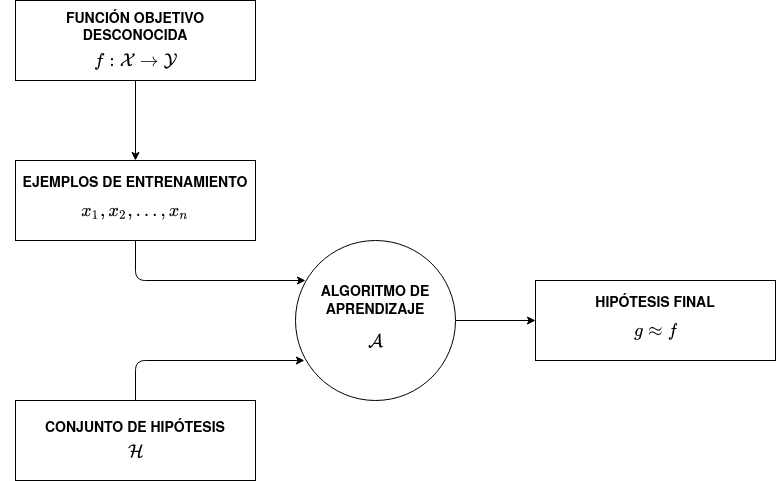
\includegraphics[width=1\textwidth]{problema-aprendizaje}
  \caption{Componentes de un problema de aprendizaje automático}
  \label{fig:problema-aprendizaje}
\end{figure}

Las tareas y experiencias pueden ser muy diversas, lo que nos permite diferenciar varios tipos de algoritmos. Según el tipo de experiencia, en general podemos diferenciar entre aprendizaje supervisado cuando al algoritmo se le proporciona un conjunto de ejemplos para los cuales la tarea está ya resuelta o no supervisado cuando el algoritmo cuenta solo con ejemplos que no están resueltos. Cuando se trabaja con ejemplos resueltos y sin resolver se trata de aprendizaje semi-supervisado, y cuando no se proporciona una respuesta a cada ejemplo pero sí se asigna una puntuación a cada posible respuesta se trata de aprendizaje por refuerzo. Algunas de las tareas a las que pueden aplicarse son:

\begin{itemize}
  \item Clasificación: el programa debe deducir a qué clase pertenece cada instancia de los datos.
  \item Regresión: el programa debe asignar un valor real a cada instancia.
  \item Síntesis y muestreo: el programa debe generar nuevos ejemplos parecidos a los usados para su entrenamiento.
\end{itemize}

Una primera aproximación a la solución de problemas de aprendizaje son los modelos lineales, como el de regresión lineal o regresión logística, modelos cuyo conjunto de hipótesis es de funciones lineales sobre el conjunto de entrada. Su principal desventaja es su limitación a la hora de aproximar funciones no lineales, ya que no son capaces de expresar las posibles interacciones entre variables.

Existen también modelos no lineales, entre los que se encuentran los modelos basados en árboles de decisióno modelos basando en distancias entre ejemplos como los $k$ vecinos más cercanos. Estos modelos sí permiten modelar relaciones no lineales entre los datos.

El aprendizaje profundo o \textit{deep learning} es una rama del aprendizaje automático basada en el uso de redes neuronales. Surge en parte como respuesta al problema de los modelos lineales, ya que permite la aproximación de funciones no lineales mediante el aprendizaje de sucesivas transformaciones no lineales de los datos de entrada. En este apartado se introducen estos modelos y su entrenamiento.

\section{Redes neuronales prealimentadas}

Las redes prealimentadas profundas, redes neuronales profundas o perceptrones multicapa, \textit{deep feedforward networks}, \textit{feedforward neural networks} o \textit{multilayer perceptron} (MLP) en inglés, son el modelo canónico del aprendizaje profundo~\cite{abu2012learning}. Su objetivo es aproximar la función $f^*$ mediante una aplicación $f(\textbf{x};\theta)$ y aprendiendo el valor de los parámetros $\theta$ que permita un mejor resultado.

Se llaman redes ya que suelen representarse componiendo varias funciones diferentes. El modelo puede asociarse con un grafo dirigido acíclico que describe cómo se componen las funciones. Un ejemplo de esta estructura es, teniendo tres funciones vectoriales $f_1$, $f_2$ y $f_3$, componerlas de la forma $f(\textbf{x}) = f_3(f_2(f_1(\textbf{x})))$. En este caso la función $f_i$ se llama capa i-ésima de la red. La longitud de la cadena es la profundidad de la red, de donde surge la nomeclatura redes profundas. La última capa de la red se llama capa de salida.

\begin{figure}[htpb]
  \centering
  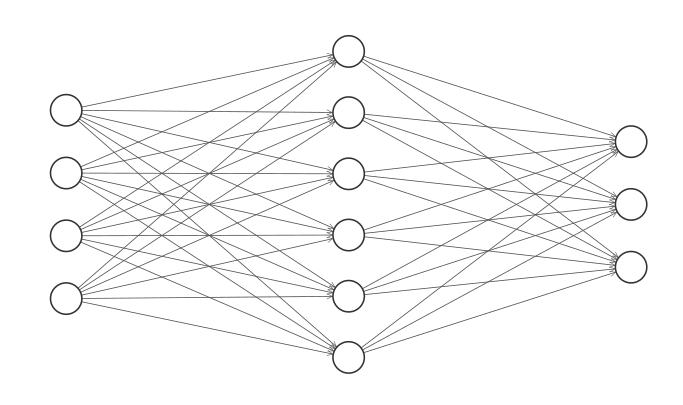
\includegraphics[width=1\textwidth]{nn}
  \caption{Ejemplo de red neuronal prealimentada de profundidad 3}
  \label{fig:nn}
\end{figure}


Durante el entrenamiento se intenta conseguir que $f(\textbf{x})$ se aproxime a $f^*(\textbf{x})$. Los datos del conjunto de entrenamiento ofrecen ejemplos, aproximados y ruidosos, de la función $f^*$ evaluada en diferentes $\textbf{x} \in \mathcal{X}$. Cada ejemplo \textbf{x} está normalmente acompañado de una salida deseada $\textbf{y} \approx f^*(\textbf{x})$. Así, los ejemplos especifican qué resultado debe ofrecer la capa de salida para cada uno de ellos. El comportamiento del resto de capas no está especificado, y es el algoritmo de aprendizaje el que debe configurarlo para obtener la mejor aproximación de $f^*$.

Que el grafo sea acíclico implica que no existe retroalimentación con la salida de ninguna de las unidades de la red. Cuando el modelo se extiende para permitir la retroalimentación se trata de una red neuronal recurrente, que veremos posteriormente.

El componente básico de cada una de las capas, al que llamamos unidad, consiste en una función de $\mathbb{R}^n$ en $\mathbb{R}$, donde $n$ es el tamaño de la capa anterior. Cada unidad recibe la salida de las unidades de la capa anterior y calcula un valor que devuelve, su valor de activación. Este comportamiento se inspira en las neuronas biológicas ~\cite{izenman2008modern}, por eso este tipo de modelos recibe el nombre de red neuronal.

Puesto que el objetivo es aproximar funciones no lineales, no basta con que las transformaciones que aplican estas unidades sean transformaciones lineales de los datos de entrada. De ser así, podríamos resumir el comportamiento de la red al completo en una única transformación lineal. Se busca por tanto el aprendizaje de una transformación no lineal $\phi$ de entre una clase de funciones parametrizadas. Se define así un modelo del tipo $$y = f(\textbf{x};\theta,\textbf{w}) = \phi(\textbf{x};\theta)^T\textbf{w}$$ donde $\theta$ es un vector de parámetros que permite seleccionar $\phi$ de entre la familia que elegimos y $w$ se utiliza para aplicar la transformación de los datos obtenida en la salida deseada. La clase de funciones de entre los que el modelo busca la aproximación, el conjunto de hipótesis, se determina al seleccionar la estructura de la red y los tipos de unidades ocultas y de salida.


\subsection{Función de coste}

La mayoría de diseños de redes neuronales se realizan definiendo la distribución $P(y|x;\theta)$ y aplicando el principio de máxima verosimilitud. Si $\textbf{X} = \{\textbf{x}_1,...,\textbf{x}_n\}$ representa los ejemplos, $\textbf{Y} = \{\textbf{y}_1,...,\textbf{y}_n\}$ sus soluciones, el estimador de máxima verosimilitud vendrá dado por $$\theta_{ML} = \arg \max_{\theta} P(\textbf{Y}|\textbf{X}; \theta).$$
Asumiendo que los ejemplos son independientes e idénticamente distribuidos
$$\theta_{ML} = \arg \max_{\theta} \prod_{i=1}^n P(\textbf{y}_i|\textbf{x}_i; \theta).$$

Puesto que el logaritmo es una función estrictamente creciente, tomar el logaritmo nos da un problema de optimización equivalente, por lo que $$\theta_{ML} = \arg \max_{\theta} \sum_{i=1}^n \log P(\textbf{y}_i|\textbf{x}_i; \theta).$$

Escalar la función tampoco cambia cuál es el máximo, por lo que podemos dividir entre $n$ para obtener una expresión respecto de la esperanza de la distribución empírica $\hat{P}_{\text{data}}$ de los datos de entrenamiento

$$\theta_{ML} = \frac{1}{n} \arg \max_{\theta} \sum_{i=1}^n \log P(\textbf{y}_i|\textbf{x}_i; \theta) = \mathbb{E}_{\textbf{x}, \textbf{y} \sim \hat{P}_{\text{data}}}\log P(\textbf{y}|\textbf{x}).$$

Teniendo esto, podemos definir la función de coste como
$$J(\theta) = -\mathbb{E}_{\textbf{x}, \textbf{y} \sim \hat{P}_{\text{data}}}\log P(\textbf{y}|\textbf{x}).$$

La expresión concreta de la función de coste cambia con el modelo, dependiendo de la distribución $P$. Normalmente también se añade un término de regularización. Con este, la función de coste es de la forma
$$J(\theta) = -\mathbb{E}_{\textbf{x}, \textbf{y} \sim \hat{P}_{\text{data}}}\log P(\textbf{y}|\textbf{x}) + \lambda \Omega (\theta).$$

\subsection{Unidades de salida}

Siguiendo el método previo, la elección de la representación de la salida de una red prealimentada determina la expresión de su función de coste. En esta sección estudiamos qué tipo de unidades suelen utilizarse como salida de la red. Para ello supondremos que las unidades ocultas nos proporcionan un vector de características $\textbf{h} = f(\textbf{x};\theta)$. La capa de salida transforma estas características para completar la tarea que la red debe cumplir.

\subsubsection{Unidades lineales}

Dadas las características $\textbf{h}$, una capa con unidades lineales produce un vector $\textbf{y} = \textbf{W}^T \textbf{h} + \textbf{b}$, sin transformaciones no lineales. Suelen usarse para producir la media de una distribución condicional normal $$p(\textbf{y}|\textbf{x}) = \mathcal{N}(\textbf{y}^*; \textbf{y},I).$$ En este caso obtener la máxima verosimilitud equivale a minimizar el error cuadrático medio.

\subsubsection{Unidades con activación sigmoidal}

Muchas tareas requieren predecir una variable binaria $y$. Un ejemplo de ello son los problemas de clasificación con dos clases. En este caso la aproximación del método de máxima verosimilitud es definir una distribución de Bernouilli sobre $y$ condicionada a $\textbf{x}$. La red neuronal tendrá entonces que predecir $P(y=1| \textbf{x})$. El número generado por la red, por tanto, estará en el intervalo $[0,1]$.

Para un correcto entrenamiento mediante técnicas basadas en gradiente es necesario que no genere un gradiente nulo o muy cercano a $0$ cuando el modelo no se acerque a la solución. Para ello se aplica una función de activación sigmoidal a la salida, como la función logística $$y = \sigma (\textbf{w}^T\textbf{h} + b) = \frac{1}{1 + e^{-(\textbf{w}^T\textbf{h} + b)}}.$$

Definamos entonces una distribución de probabilidad sobre $y$ usando el valor de $z = \textbf{w}^T\textbf{h} + b$. La elección de la función de activación sigmoidal puede justificarse construyendo una distribución de probabilidad no normalizada $\hat{P}$(y), cuya suma no es 1, que supondremos $\log$-lineal en $z$ e $y$. Entonces podemos exponenciar para obtener una distribución de probabilidad válida y normalizando obtendremos una distibución de Bernouilli controlada por una transformación sigmoidal de $z$:

$$\log \hat{P}(y) = yz$$ $$\hat{P}(y) = e^{yz}$$ \\ $$P(y) = \frac{e^{yz}}{e^{0z}+e^{1z}} = \frac{e^{yz}}{1+e^z} = \sigma((2y-1)z). $$

De esta manera la función de coste es $$J(\theta) = -\log P(y|\textbf{x}) = - \log \sigma((2y-1)z).$$ Esta función solo se satura cuando $y = 1$ y $z$ es muy positivo o cuando $y = 0$ y $z$ es muy negativo, es decir, cuando el modelo alcanza la respuesta. Esta función está bien definida ya que cualquier función sigmoidal toma valores en $(0,1)$, y por tanto el logaritmo es finito.

\subsubsection{Unidades softmax}

La función de activación softmax puede utilizarse para representar una distribución de probabilidad sobre una variable discreta con $n$ valores posibles. Este es el caso de los problemas de clasificación con más de dos clases. Puede interpretarse por tanto como una generalización para las funciones de activación sigmoidal.

En este caso se necesita generar un vector $\textbf{y}$, con $y_i = P(y = i| \textbf{x})$. Cada elemento de $\textbf{y}$ debe estar en $[0,1]$, y la suma de todos ellos debe ser 1 para representar una distribución de probabilidad válida.

Siguiendo el razonamiento anterior, una capa lineal predice probabilidades logarítmicas no normalizadas, $$\textbf{z} = \textbf{W}^T \textbf{h} + b$$ donde $z_i = \log \hat{P}(y = i | \textbf{x})$. La función softmax, definida componente a componente como $$\text{softmax}(\textbf{z})_i = \frac{e^{z_i}}{\sum_j e^{z_j}}, $$  exponencia y normaliza $\textbf{z}$ para obtener la $\textbf{y}$ deseada. Igual que en el caso anterior, la función de coste puede obtenerse aplicando el principio de máxima verosimilitud.

\subsection{Unidades ocultas}\label{unidades-ocultas}

Cualquiera de los tipos de unidad anterior puede utilizarse en una capa oculta, pero existen más diseños. En este apartado se describen algunos de los tipos más comunes. Por lo general, las capas ocultas aceptan un vector de entrada $\textbf{x}$ sobre el que realizan una transformación afín $\textbf{z} = \textbf{W}^T\textbf{x} + \textbf{b}$, donde la matriz $\textbf{W}$ se llama matriz de pesos y el vector $\textbf{b}$ vector de sesgo, y después aplican una transformación no lineal $g(\textbf{z})$, llamada función de activación. La elección de esta transformación es la que marca el tipo de unidad que se selecciona.

Algunas de las unidades ocultas aquí expuestas no son diferenciables en todos los puntos. Podría parecer que esto las invalida para el aprendizaje mediante métodos de gradiente. En la práctica el descenso del gradiente funciona bien con estas funciones de activación ya que no se suele llegar a un mínimo de la función de coste, sino reducir su valor. Por ello no se obtendrá un valor en el que el gradiente sea nulo, y es aceptable que el mínimo de la función de coste corresponda a valores en los que el gradiente no está definido. Por lo tanto, en la práctica, pueden no tenerse en cuenta los puntos en los que las funciones aquí descritas no son diferenciables.

\subsubsection{Unidades lineales rectificadas}\label{unidades-relu}

Las unidades lineales rectificadas (\textit{ReLU}) utilizan la función de activación $g(\textbf{z})_i = \max\{0,z_i\}$.

\begin{figure}[htpb]
  \centering
  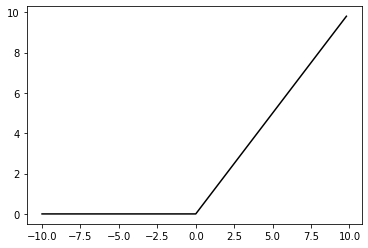
\includegraphics[width=0.6\textwidth]{relu}
  \caption{Gráfica de la función \textit{ReLU}}
  \label{fig:relu}
\end{figure}

Estas unidades son fáciles de optimizar por su parecido a las unidades lineales. La única diferencia con estas es que las rectificadas se anulan en la mitad de su dominio. Existen múltiples generalizaciones de este tipo de unidades:

\begin{itemize}
\item Rectificación mediante valor absoluto: $g(\textbf{z})_i = \lvert z_i \rvert$.
\item Leaky \textit{ReLU}: $g(\textbf{z})_i = \max \{0,z_i\} + \alpha \min \{0,z_i\}$ con un $\alpha$ fijo, normalmente $0,01$.
\item \textit{ReLU} paramétríca: $g(\textbf{z})_i = \max\{0,z_i\} + \alpha_i \min \{0,z_i\}$ con $\alpha_i$ un parámetro optimizable.
\end{itemize}

\begin{figure}[htpb]
  \centering
  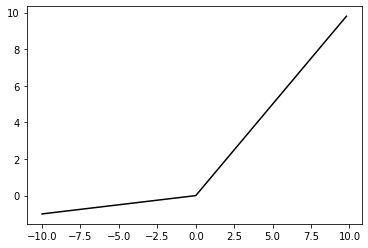
\includegraphics[width=0.6\textwidth]{leakyrelu}
  \caption{Gráfica de la función \textit{leaky ReLU} con $\alpha = 0,1$}
  \label{fig:leakyrelu}
\end{figure}


Otra generalización importante son las unidades maxout, que agrupa los elementos de $z$ en subconjuntos de $k$ elementos. Cada una de las unidades de una capa de este tipo devuelve el máximo de uno de estos subconjuntos. Así,

$$ g(\textbf{z})_i = \max_{j \in \mathbb{G}(i)} z_j$$

donde $\mathbb{G}(i) = \{(i-1)k +1,...,ik\}$ es el conjunto de índices para el subconjunto $i$-ésimo. Una capa de estas unidades puede aprender una función convexa lineal a trozos de hasta $k$ trozos. Podemos considerar que más que la relación entre las unidades, estas capas aprenden la función de activación misma. Con un $k$ suficientemente grande, estas unidades pueden aprende a aproximar cualquier función convexa con precisión arbitraria~\cite{goodfellow2016}.

\subsubsection{Unidades con activación sigmoidal}

Otras dos unidades comunes utilizan funciones sigmoidales, la función logística

$$g(\textbf{z})_i = \sigma(z_i) = \frac{1}{1+e^{-z_i}}$$

\begin{figure}[htpb]
  \centering
  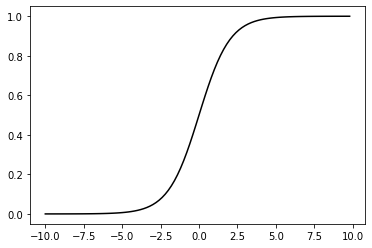
\includegraphics[width=0.6\textwidth]{logistica}
  \caption{Gráfica de la función logística}
  \label{fig:logistica}
\end{figure}

y la función tangente hiperbólica

$$g(\textbf{z})_i = \tanh(z_i) = \frac{e^{z_i} - e^{-z_i}}{e^{z_i}+e^{-z_i}}.$$

\begin{figure}[htpb]
  \centering
  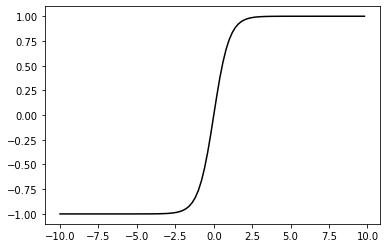
\includegraphics[width=0.6\textwidth]{tanh}
  \caption{Gráfica de la función tangente hiperbólica}
  \label{fig:tanh}
\end{figure}

Estas dos funciones están muy relacionadas, ya que $\tanh (z) = 2 \sigma (2z) - 1$. Las funciones sigmoidales se saturan en gran parte de su dominio, lo que puede dificultar el aprendizaje. Es por ello que su uso ha disminuido desde la introducción de las \textit{ReLU}.

\subsection{Propagación hacia adelante}

Una vez configurada la red, esta recibe una entrada que se propaga a través de cada una de las capas, que le aplican las transformaciones correspondientes hasta la salida. Este proceso se llama propagación hacia adelante, y se describe en el algoritmo \ref{feedforward-propagation}.


\begin{algorithm}
\label{feedforward-propagation}
 \caption{Propagación hacia adelante en una red neuronal profunda con función de activación $g$ para una entrada \textbf{x}.}
     \SetAlgoLined
     \KwIn{$\ell$ profundidad de la red}
     \KwIn{$\textbf{W}_i$ matriz de pesos de la capa $i$-ésima, $i = 1,...,\ell$}
     \KwIn{$\textbf{b}_i$ vector de sesgos de la capa $i$-ésima, $i = 1,...,\ell$}
     \KwIn{$\textbf{x}$ entrada de la red}
     $\textbf{h}_0 \leftarrow \textbf{x}$\;
     \For{$i = 1,...,\ell$}{
      $\textbf{z}_i \leftarrow (\textbf{W}_{i})^T\textbf{x}_{i-1} + \textbf{b}_i$\;
      $\textbf{h}_i \leftarrow g_i(\textbf{z}_i)$\;
     }
     $\textbf{y} \leftarrow \textbf{h}_{\ell}$\;
\end{algorithm}


\section{Entrenamiento de redes neuronales prealimentadas}

\subsection{Optimización}\label{optimizacion}

Una vez conocida la función de coste $J(\theta)$ el siguiente paso es buscar unos parámetros $\theta$ que la minimicen. Para resolver este problema de optimización, al menos de forma aproximada, se aplica la técnica del descenso del gradiente. Este método fue inicialmente propuesto por Cauchy~\cite{cauchy1847methode} en 1847 y su convergencia fue estudiada por primera vez por Curry~\cite{curry1944method} en 1944.

\subsubsection{Descenso del gradiente}

Sea $f$ un campo escalar de $S \subset \mathbb{R}^n$ en $\mathbb{R}$, continuo en $S$ y derivable con derivada continua en el interior de $S$. La dirección en la que la función desciende más rápidamente vendrá dada por la del vector $$- \varepsilon \nabla f(x_1,...x_n) = \left( -\varepsilon \frac{\partial f}{\partial x_1}(x_1,...,x_n), ..., - \varepsilon \frac{\partial f}{\partial x_n}(x_1,...,x_n) \right),$$ donde $\varepsilon > 0$ es un factor de proporcionalidad al que suele llamarse tasa de aprendizaje. El método consiste en, desde un punto inicial $\textbf{x}_0$ e iterativamente, calcular el opuesto del gradiente y avanzar en esa dirección una distancia determinada por $\varepsilon$. Así, en la iteración $i$-ésima, $\textbf{x}^{(i)} = \textbf{x}^{(i-1)} - \varepsilon \nabla f(\textbf{x}^{(i-1)})$.  El algoritmo termina cuando el valor de $\nabla f(x_1,...,x_n)$ es cercano a cero, con una tolerancia dada.

La convergencia del proceso al mínimo está probada cuando el mínimo de la función sobre la que se aplica es único. Este no es el caso de las funciones a las que se aplica en el contexto del aprendizaje profundo. Las funciones de coste que se intentan optimizar pueden tener muchos mínimos locales o puntos de silla en los que el algoritmo puede terminar sin obtener una buena solución. Otro inconveniente importante es el coste computacional que supone la aplicación del algoritmo a muestras grandes de datos, como suele hacerse en el aprendizaje automático para obtener modelos suficientemente generales. Es por ello que en la práctica se utilizan versiones del procedimiento que responden a estas cuestiones.

\subsubsection{Descenso del gradiente estocástico (SGD)}

La aplicación del descenso del gradiente a un problema de aprendizaje automático se realiza calculando la media aritmética de los gradientes de la función de pérdida para cada uno de los datos del conjunto de entrenamiento. Esto implica evaluar la función de coste para cada ejemplo del conjunto de entrenamiento antes de actualizar el gradiente, lo que puede ser computacionalmente inasumible. Es por ello que en la actualidad la técnica más usada es una aproximación en la que se utiliza un solo ejemplo para cada actualización. Este es, en la actualidad, el algoritmo más utilizado. Se describe detalladamente en \ref{sgd}.

\begin{algorithm}
\label{sgd}
 \caption{Algoritmo de descenso del gradiente estocástico.}
     \SetAlgoLined
     \KwIn{$\theta$ vector inicial de parámetros}
     \KwIn{$\varepsilon$ tasa de aprendizaje}
     \KwIn{$\textbf{x}_1,...,\textbf{x}_n$ ejemplos de entrenamiento}
     \KwIn{$\textbf{y}_1,...,\textbf{y}_n$ objetivo de cada ejemplo}
     \While{no se alcanza un mínimo aproximado}{
      Mezclar aleatoriamente los ejemplos del conjunto de entrenamiento\;
      \For{$i = 1,...,n$}{
        $\theta \leftarrow \theta - \varepsilon \nabla L( f(\textbf{x}_i; \theta),\textbf{y}_i)$\;
      }
     }
\end{algorithm}

\subsubsection{Variantes de SGD}

Mediante la aplicación de SGD se mitiga el problema del coste computacional del descenso del gradiente, pero la posibilidad de terminar en un mínimo local no óptimo o en un punto de silla sigue existiendo. Además, la aproximación que realiza SGD del gradiente puede no ser suficientemente buena. Existen diferentes alternativas que afrontan estos problemas.

\begin{itemize}
\item Gradiente descendente estocástico con minilotes: para realizar una aproximación más fiel del gradiente de la función toma minilotes de elementos del conjunto de entrenamiento en lugar de un solo elemento. Se describe detalladamente en \ref{sgd-minilotes}.
\item Método del momento~\cite{sutskever2013training}: en cada paso se recuerda la anterior actualización y la siguiente se calcula como una combinación lineal entre esta y el gradiente. De esta manera la variación de la dirección de una iteración a otra disminuye, evitando el comportamiento de zigzagueo. Se describe detalladamente en \ref{momentum}.
\item AdaGrad~\cite{duchi2011adaptive}: se basa en adaptar la tasa de aprendizaje para cada parámetro de forma inversamente proporcional a la raíz cuadrada de la suma de los valores anteriores. Así se decrementa más rápidamente la tasa de aprendizaje para los parámetros con mayor derivada parcial y se progresa más rápidamente en las zonas de menor pendiente. Se describe detalladamente en \ref{adagrad}.
\item RMSProp~\cite{tieleman2012lecture}: similar a adagrad, modifica la tasa de aprendizaje para cada parámetro. En este caso se cambia la acumulación del gradiente por una media con pesos exponenciales para mejorar su comportamiento en funciones no convexas. Se describe detalladamente en \ref{rmsprop}.
\item Adam~\cite{kingma2014adam}: es otro algoritmo con tasa de aprendizaje adaptativa. Es una combinación entre RMSProp y método del momento, ya que añade un momento adaptativo. Se describe detalladamente en \ref{adam}.
\end{itemize}

\begin{algorithm}
\label{sgd-minilotes}
 \caption{Algoritmo de descenso del gradiente estocástico con minilotes.}
     \SetAlgoLined
     \KwIn{$\theta$ vector inicial de parámetros}
     \KwIn{$m$ tamaño de minilote}
     \KwIn{$\varepsilon$ tasa de aprendizaje}
     \KwIn{$\textbf{x}_1,...,\textbf{x}_n$ ejemplos de entrenamiento}
     \KwIn{$\textbf{y}_1,...,\textbf{y}_n$ objetivo de cada ejemplo}
     \While{no se alcanza un mínimo aproximado}{
      Seleccionar un minilote de $m$ ejemplos del conjunto de entrenamiento $\{\textbf{x}_1,...,\textbf{x}_m\}$ y sus correspondientes objetivos $\textbf{y}_i$\;
        $\theta \leftarrow \theta - \frac{\varepsilon}{m} \nabla \sum_i L( f(\textbf{x}_i; \theta),\textbf{y}_i)$\;

     }
\end{algorithm}

\begin{algorithm}
\label{momentum}
 \caption{SGD con método del momento.}
     \SetAlgoLined
     \KwIn{$\theta$ vector inicial de parámetros}
     \KwIn{$\varepsilon$ tasa de aprendizaje}
     \KwIn{$\alpha$ valor del momento}
     \KwIn{$v$ velocidad inicial}
     \KwIn{$\textbf{x}_1,...,\textbf{x}_n$ ejemplos de entrenamiento}
     \KwIn{$\textbf{y}_1,...,\textbf{y}_n$ objetivo de cada ejemplo}
     \While{no se alcanza un mínimo aproximado}{
     Seleccionar un minilote de $m$ ejemplos del conjunto de entrenamiento $\{\textbf{x}_1,...,\textbf{x}_m\}$ y sus correspondientes objetivos $\textbf{y}_i$\;
     $v \leftarrow \alpha v - \frac{\varepsilon}{m} \nabla \sum_i L( f(\textbf{x}_i; \theta),\textbf{y}_i)$\;
     $\theta \leftarrow \theta + v$\;

     }
\end{algorithm}

\begin{algorithm}
\label{adagrad}
 \caption{Adagrad. $\odot$ representa el producto componente a componente, $\sqrt{\cdot}$ la raíz cuadrada componente a componente y la división $\frac{\varepsilon}{\delta + \sqrt{r}}$ se realiza componente a componente.}
     \SetAlgoLined
     \KwIn{$\theta$ vector inicial de parámetros}
     \KwIn{$\delta$ constante pequeña, normalmente $10^{-6}$}
     \KwIn{$\varepsilon$ tasa de aprendizaje inicial}
     \KwIn{$\textbf{x}_1,...,\textbf{x}_n$ ejemplos de entrenamiento}
     \KwIn{$\textbf{y}_1,...,\textbf{y}_n$ objetivo de cada ejemplo}
     $r \leftarrow 0$\;
     \While{no se alcanza un mínimo aproximado}{
      Seleccionar un minilote de $m$ ejemplos del conjunto de entrenamiento $\{\textbf{x}_1,...,\textbf{x}_m\}$ y sus correspondientes objetivos $\textbf{y}_i$\;
        $g \leftarrow \frac{1}{m} \nabla \sum_i L( f(\textbf{x}_i; \theta),\textbf{y}_i)$\;
        $r \leftarrow r + g \odot g$\;
        $\theta \leftarrow \theta - \frac{\varepsilon}{\delta + \sqrt{r}} \odot g$\;
     }
\end{algorithm}

\begin{algorithm}
\label{rmsprop}
 \caption{RMSProp. $\odot$ representa el producto componente a componente, $\sqrt{\cdot}$ la raíz cuadrada componente a componente y la división $\frac{\varepsilon}{\delta + \sqrt{r}}$ se realiza componente a componente.}
     \SetAlgoLined
     \KwIn{$\theta$ vector inicial de parámetros}
     \KwIn{$\rho$ ratio de decaimiento}
     \KwIn{$\delta$ constante pequeña, normalmente $10^{-6}$}
     \KwIn{$\varepsilon$ tasa de aprendizaje inicial}
     \KwIn{$\textbf{x}_1,...,\textbf{x}_n$ ejemplos de entrenamiento}
     \KwIn{$\textbf{y}_1,...,\textbf{y}_n$ objetivo de cada ejemplo}
     $r \leftarrow 0$\;
     \While{no se alcanza un mínimo aproximado}{
      Seleccionar un minilote de $m$ ejemplos del conjunto de entrenamiento $\{\textbf{x}_1,...,\textbf{x}_m\}$ y sus correspondientes objetivos $\textbf{y}_i$\;
        $g \leftarrow \frac{1}{m} \nabla \sum_i L( f(\textbf{x}_i; \theta),\textbf{y}_i)$\;
        $r \leftarrow \rho r + (1 - \rho) g \odot g$\;
        $\theta \leftarrow \theta - \frac{\varepsilon}{\delta + \sqrt{r}} \odot g$\;
     }
\end{algorithm}

\begin{algorithm}
\label{adam}
 \caption{Adam. $\odot$ representa el producto componente a componente, $\sqrt{\cdot}$ la raíz cuadrada componente a componente y la división $\frac{\varepsilon}{\delta + \sqrt{r}}$ se realiza componente a componente.}
     \SetAlgoLined
     \KwIn{$\theta$ vector inicial de parámetros}
     \KwIn{$\rho_1, \rho_2 \in [0,1)$ ratios de decaimeiento exponencial, sugeridos por defecto $0,9$ y $0,99$}
     \KwIn{$\delta$ constante pequeña, normalmente $10^{-6}$}
     \KwIn{$\varepsilon$ tasa de aprendizaje inicial}
     \KwIn{$\textbf{x}_1,...,\textbf{x}_n$ ejemplos de entrenamiento}
     \KwIn{$\textbf{y}_1,...,\textbf{y}_n$ objetivo de cada ejemplo}
     $r \leftarrow 0$\;
     $s \leftarrow 0$\;
     $t \leftarrow 0$\;
     \While{no se alcanza un mínimo aproximado}{
      Seleccionar un minilote de $m$ ejemplos del conjunto de entrenamiento $\{\textbf{x}_1,...,\textbf{x}_m\}$ y sus correspondientes objetivos $\textbf{y}_i$\;
        $g \leftarrow \frac{1}{m} \nabla \sum_i L( f(\textbf{x}_i; \theta),\textbf{y}_i)$\;
        $t \leftarrow t+1$\;
        $r \leftarrow \rho_1 r + (1 - \rho_1) g$\;
        $r \leftarrow \rho_2 r + (1 - \rho_2) g \odot g$\;
        $\hat{s} \leftarrow \frac{s}{1 - \rho_1^t}$\;
        $\hat{r} \leftarrow \frac{s}{1 - \rho_2^t}$\;
        $\theta \leftarrow \theta - \frac{\hat{s}}{\sqrt{\hat{r}}+\delta} \odot g$\;
     }
\end{algorithm}

\subsection{Propagación hacia atrás}\label{back-propagation}

El cálculo del gradiente de la función de coste es básico para el entrenamiento de redes neuronales. Obtener su expresión analítica es sencillo, pero evaluar numéricamente esa expresión puede ser muy costoso computacionalmente. El algoritmo de propagación hacia atrás (\textit{back propagation}) permite realizar este cálculo de manera eficiente, utilizando la regla de la cadena para evitar repetir el cálculo de derivadas parciales que aparecen varias veces en el proceso.

Tras aplicar propagación hacia adelante se aplica el algoritmo descrito en \ref{backprop}, que obtiene los gradientes de la función de activación de cada capa, empezando por la capa de salida y yendo hacia atrás hasta la primera capa oculta. De estos gradientes, que pueden ser interpretados como la indicación de cómo la salida de cada capa debería cambiar para reducir el error, se puede obtener el gradiente respecto de los parámetros de cada capa. Obtenido el gradiente respecto de los pesos y los sesgos, puede utilizarse para aplicar alguno de los métodos de optimización basados en gradiente.

\begin{algorithm}
\label{backprop}
 \caption{Propagación hacia atrás con entrada $\textbf{x}$, salida $\textbf{y}$, objetivo $\textbf{y}^*$ y profundidad $\ell$. $L$ representa la función de coste sin regularización, y $J$ la función de coste completa. $\odot$ denota el producto componente a componente.}
     \SetAlgoLined
     $\textbf{d} \leftarrow \nabla_\textbf{y} J(\textbf{y},\textbf{y}^*;\theta) = \nabla_\textbf{y} L(\textbf{y},\textbf{y}^*)$\;
     \For{$k = \ell,...,1$}{
      $\textbf{d} \leftarrow \nabla_{\textbf{z}_k} J = \textbf{d} \odot g'(\textbf{z}_k)$\;
      $\nabla_{\textbf{b}_k} J = \textbf{d} + \lambda \nabla_{\textbf{b}_k} \Omega(\theta)$\;
      $\nabla_{\textbf{W}_k} J = \textbf{d}(h_{k-1})^T + \lambda \nabla_{\textbf{W}_k} \Omega(\theta)$\;
      $\textbf{d} \leftarrow \nabla_{h_{k-1}}J = (\textbf{W}_k)^T \textbf{d}$\;
     }

\end{algorithm}

\endinput
%------------------------------------------------------------------------------------
% FIN DEL CAPÍTULO.
%------------------------------------------------------------------------------------
